\documentclass{article}

% Language setting
% Replace `english' with e.g. `spanish' to change the document language
\usepackage[english]{babel}
\usepackage{geometry}
\usepackage{algorithm}
\usepackage[noend]{algpseudocode}

% Set page size and margins
% Replace `letterpaper' with `a4paper' for UK/EU standard size
 \geometry{
 a4paper,
 total={170mm,257mm},
 left=20mm,
 top=20mm,
 }
% Useful packages
\usepackage{amsmath}
\usepackage{amssymb}

\usepackage{graphicx}
\usepackage[colorlinks=true, allcolors=blue]{hyperref}



\title{Reasoning and Agents}
\author{Finlay Ross-Davie}
\date{17th January 2024}

\begin{document}
\maketitle


\section{Intelligent Agents}

\subsection{Definition of agents and environments}

An \textbf{Agent} is anything that can be viewed as perceiving its environment through \textbf{sensors} and acting upon that environment through \textbf{actuators} \newline. 

\textbf{Percept} is a term used to refer to the agent's perceptual inputs at any given instant. An agent's 

\textbf{percept sequence} is the complete history of everything the agent has ever perceived \newline

An agent's choice of action at any given instant can depend on the entire percept sequence observed, but not anything it hasn't perceived.

An agent's behavior is described, mathematically speaking, by the \textbf{agent function} that maps any given percept sequence to an action.

The agent function for an artificial agent will be implemented by an \textbf{agent program}.

i.e, The agent program is an abstract mathematical description; the agent program is a concrete implementation, running within some physical system 

\subsection{The Concept of rationality}

A \textbf{performance measure} evaluates any given sequence of environment states to capture whether the agent has performed well.

In general, it is better to design performance measures according too what one actually wants in the environment, rather than according to how one thinks the agent should behave. \newline

What is rational at any given time depends on four things:

\begin{itemize}
    \item The performance measure that defined the criterion of success
    \item The agents prior knowledge of the environment
    \item The actions that the agent can perform
    \item The agent's percept sequence to date.

\end{itemize}

The definition of a \textbf{rational agent}:

For each possible percept sequence, a rational agent should select an action that is expected to maximize its performance measure, given the evidence provided by the percept sequence and whatever built in knowledge the agent has. \newline

An \textbf{omniscient} agent knows the actual outcome of its actions and can act accordingly; but omniscience is impossible in reality.

Rationality maximises expected performance

To the extent that an agent relies on the prior knowledge of its designer rather than on its own percepts, we can say that the agent lacks \textbf{autonomy}. A rational agent should be autonomous - it should learn what it can to compensate for a partial or incorrect prior knowledge

The \textbf{task environment} is made up of  the performance measure, the environment, and the agent's actuators and sensors. This is also referred to as the \textbf{PEAS} (Performance, Environment, Actuators, Sensors) description \newline

If an agent's sensors give it access to the complete state of the environment at each point in time, then one can say that the task environment is \textbf{Fully observable}. A task environment is effectively fully observable if the sensors detect all aspects that are relevant to the choice of action; relevance, in turn depends on the performance measure. An environment might be \textbf{partially observable} because of noisy and inaccurate sensors or because parts of the state are simply missing from the sensor data \newline

If the next state of the environment is completely determined by the current state and the action executed by the agent, the environment is \textbf{deterministic}; otherwise it is \textbf{stochastic}. \newline

In an \textbf{episodic} task environment, the agent's experience is divided into atomic episodes. In each episode the agent receives a percept and then performs a single action. The next action does not depend on the actions taken in previous episodes. In \textbf{sequential} environments, the current decision could affect all future decisions. \newline 

If the environment can change while an agent is deliberating then the environment is \textbf{dynamic} for that agent, otherwise it is \textbf{static}. \newline

In a \textbf{known} environment, the outcomes (or outcome probabilities if the environment is stochastic) for all actions are given. If an environment is \textbf{unknown} the agent will have to learn how it works in order for it to make good decisions.

\subsection{The structure of agents}

agent = architecture + program

Where \textbf{architecture} is some sort of computing device with physical sensors and actuators.

Agent programs simply take the current percept as input from the sensors and return an action to the actuators. If the agent's actions need to depend on the entire percept sequence, the agent will hve to remember the percepts.

One kind of agent is the \textbf{simple reflex agent}. These agents select actions on the basis of the current percept, ignoring the rest of percept history. \

A \textbf{model} is a description of how the next state depends on the current state and action. A \textbf{model-based agent} is an agent that uses a model to keep track of the current state of the world, then chooses an action in the same way as the reflex agent. \newline

\textbf{Goal} information describes situations that are desirable. For \textbf{Goal based agents} the agent combine program will combine this goal information with the model to choose actions that achieve the goal. \newline

Goals alone are not enough to generate high-quality behaviour in most environments. An agent's \textbf{utility function} is essentially an internalization of the performance measure. If the internal utility function and the external performance measure are in agreement, then an agent that chooses actions to maximise its utility will be rational according to the external performance measure. A rational \textbf{utility-based} agent chooses the action that maximises the expected utility of the action outcomes. \newline

All agents can improve their performance through \textbf{learning}. A \textbf{learning agent} can be divided into four conceptual components:
\begin{itemize}
    \item Critic - Provides feedback to learning element
    \item Learning element - Responsible for making improvements
    \item Problem generator - Responsible for suggesting actions that will lead to new and informative experiences
    \item Performance element - Responsible for selecting external actions
\end{itemize}

\section{Search Problems}

A search strategy is defined by picking the order of node expansion
Nodes are taken from the frontier. 

\subsection{Uninformed search}

\textbf{Uninformed search} strategies have no additional information about states beyond that provided in the problem definition. 

\subsubsection{Breadth-first search}

Breadth-first search is a strategy in which all the nodes are expanded at a given depth in the search tree before any nodes at the next level are expanded. 

This is implemented by using a FIFO queue for the frontier. This leads to new nodes going to the back of the queue, and old nodes, getting expanded first. 

This search strategy:
\begin{itemize}
    \item Is \textbf{Complete} is b is finite
    \item Has \textbf{time complexity} of $b+b^2+b^3 \ldots +b^d = O(b^d)$ in the worst case
    \item Has \textbf{space complexity} of $O(b^d)$ since it keeps every node in memory
    \item Is \textbf{Optimal} if cost = 1 per step
\end{itemize}

\subsubsection{Depth-first search}

Depth-first search is a strategy in which the deepest unexpanded node is expanded. 
This is implemented using a LIFO queue. This leads to new successors going at the front. 

This search strategy:
\begin{itemize}
    \item Is \textbf{not complete} since it fails in infinite-depth and spaces with loops
    \item Has \textbf{time complexity} of $O(b^m)$ 
    \item Has \textbf{space complexity} of $O(bm)$ linear since explored nodes with no descendants in the frontier are removed from memory
    \item Is \textbf{not optimal}
\end{itemize}

\textbf{Depth-limited} search is a implementation with a depth limit l, i.e., nodes at depth l have no successors

This search strategy:
\begin{itemize}
    \item Is \textbf{not complete} 
    \item Has \textbf{time complexity} of $O(b^l)$ 
    \item Has \textbf{space complexity} of $O(bl)$ linear since explored nodes with no descendants in the frontier are removed from memory
    \item Is \textbf{not optimal}
\end{itemize}

\subsubsection{Iterative deepening search}

Iterative deepening search is a strategy used in combination with depth-first search, that finds the best depth limit. It gradually increases the limit (0, 1,..) until a goal is found. This will occur when the depth limit reaches d, the depth of the shallowest goal node. . 

This search strategy:
\begin{itemize}
    \item Is \textbf{complete} 
    \item Has \textbf{time complexity} of $O(b^d)$ 
    \item Has \textbf{space complexity} of $O(bd)$
    \item Is \textbf{optimal} if step cost is 1
\end{itemize}

\subsection{Informed Search}

An informed search strategy is one that uses problem-specific knowledge beyond the definition of the problem itself.

\textbf{Best-first search} is an instance of the general TREE-SEARCH or GRAPH SEARCH algorithm. In best-first search a node is selected for expansion based on an \textbf{evaluation function}, $f(n)$, the evaluation function is construed as a cost estimate so the node with the lowest evaluation is expanded first. 
Most best-first algorithms include a \textbf{heuristic function}, $h(b)$. $h(n)$ estimates the cost of the cheapest path from state at node n to a goal state.  

A heuristic $h(n)$ is \textbf{admissible} if for every node n: $$h(n) \leq h^*(n)$$ where $h^*(n)$ is the true cost to reach the goal state from n 

An admissible heuristic never overestimates the cost to reach the goal i.e., it is optimistic. 

A heuristic $h(n)$ is \textbf{consistent} if for every node n, every successor n' of n generated by any action a: $$h(n) \leq c(n, a, n') + h(n')$$ 


\subsubsection{Greedy best-first search}

Greedy best-first search tries to expand the node that is closest to the goal.

The evaluation function is simply the heuristic $$f(n) = h(n)$$

This search strategy:
\begin{itemize}
    \item Is \textbf{not complete} since it can get stuck in loops
    \item Has \textbf{time complexity} of $O(b^m)$ 
    \item Has \textbf{space complexity} of $O(b^m)$ since it keeps all nodes in memory
    \item Is \textbf{not optimal}
\end{itemize}

\subsubsection{A* Search}

A* search evaluates nodes by combining $g(n)$, the cost to reach the node, and $h(n)$, the cost to get from the node to the goal.

The evaluation function is given as $$f(n) = g(n) + h(n)$$

If $h(n)$ is admissible, A* using TREE-SEARCH is optimal

If $h(n)$ is consistent, A* using GRAPH-SEARCH is optimal \newline

This search strategy:
\begin{itemize}
    \item Is \textbf{Complete} unless there are infinitely many nodes with $f \leq f(G)$
    \item Has exponential \textbf{time complexity}
    \item Keeps all nodes in memory
    \item Is \textbf{optimal}
\end{itemize}

\subsection{Smart Search using constraints}

A \textbf{constraint satisfaction problem} consists of a set of \textbf{variables} X = ${X_1,\ldots,X_n}$, a set of \textbf{domains},$D = {D_1,\ldots,D_n}$ where each domain $D_i$ is a set of possible values for variable $X_i$ and a set of \textbf{constraints} C that specify acceptable combinations of values where each $c \in C$ consists of a \textbf{scope}, tuple of variables involved in the constraint and a \textbf{relation} that defines the values that the variables can take.

Varieties of constrains:
\begin{itemize}
    \item \textbf{Unary} constraints involve a single variable
    \item \textbf{Binary} constraints involve pairs of variables
    \item \textbf{Higher-order} constraints involve 3 or more variables
    \item \textbf{Global} constraints involve an arbitrary number of variables
\end{itemize}

A variable in a CSP is \textbf{arc-consistent} if every value in its domain satisfies the variables binary constraints. 
More formally, $X_i$ is arc-consistent with respect to another variable $X_j$ if for every value in the current domain $D_i$ there is some value in the domain $D_j$ that satisfies the binary constrain on the arc $(X_i,X_)$

All CSPs are \textbf{commutative}. A problem is commutative if the order of application of any given set of actions has no effect on the outcome. When assigning values to variables in CSPs, we reach the same partial assignment regardless of order. We only need to consider assignments to a single variable at each node

\subsubsection{Backtracking search}

The term \textbf{backtracking search} is used for a depth-first search that chooses values for one variable at a time and backtracks when a variable has no legal values left to assign.

In simple terms backtracking works by choosing a variable, assigning a value to it, and then recursively trying to solve the rest of the problem.

\begin{algorithm}
\begin{algorithmic}

\Procedure{BacktrackingSearch}{$csp$}
    \Comment{returns a solution or failure}
    \State return Backtrack($[],csp$)
\EndProcedure

\Procedure{Backtrack}{$(assignment,csp)$}

\If{$assignment$ is complete}
    \State return $assignment$
\EndIf
\State $var \leftarrow$ SELECT-UNASSIGNED-VARIABLE$(csp)$
\For{\State each value in ORDER-DOMAIN-VALUES($var,assignment,csp$)}

    \If{$value$ is consistent with $assignment$}
        \State add {$var = value$} to $assignment$
        \State $inferences \leftarrow$ INFERENCE($csp,var,value$)
        \If{$inferences \neq failure$}
            \State add $inferences$ to $assignment$
            \State $result \leftarrow $ BACKTRACK($assignment,csp$)
                    \If{$result \neq failure$}
                        \State return result
                    \EndIf
                \EndIf
            \EndIf
    \State return $result$

\EndFor

\State return $failure$

\EndProcedure

\end{algorithmic}
\end{algorithm}

Variable ordering in backtracking-search (SELECT-UNASSIGNED-VARIABLE) can be decided in various manners to garner gains in speed. The \textbf{most constrained variable} technique chooses the variable with the fewest legal values, this reduces branching. \newline

Value ordering (ORDER-DOMAIN-VALUES)can be done using various techniques such as \textbf{least constraining value} which chooses the value that rules out the fewest values in the remaining variables for a given variable. \newline 

Inference (INFERENCE) allows one to potentially detect inevitable failure early. For example, \textbf{forward checking} keeps track of remaining legal values for unassigned variables and terminates the search when any variable has no legal values. Another form of inference, \textbf{constraint propagation} repeatedly enforces constrains locally . \newline \textbf{Arc consistency} checks if there is a value for X that makes the domain of Y empty before or after each assignment. The simplest form of propagation makes each arc consistent.

The most popular algorithm to make every variable arc-consistent is called AC-3 which maintains a queue of arcs to consider. Initially, the queue contains all the arcs in the CSP. AC-3 then pops off an arbitrary arc $(X_i,X_j)$ from the queue and makes $X_i$ arc-consistent with respect to $X_j$. If this leaves $D_i$ unchanged, the algorithm just moves on to the next arc. If this makes $D_i$ smaller, then all arc $(X_k,X_i)$ where $X_k$ is a neighbor of $X_i$ are added to the queue since the change in $D_i$ might enable further reductions in the domains of $D_k$. If $D_i$ is revised down to nothing, the CSP has no consistent solution and AC-3 can return failure


\begin{algorithm}
\begin{algorithmic}

\Procedure{AC-3}{$csp$}
    \Comment{returns false if an inconsistency is found and true otherwise}
    \While{queue is not empty}
        \State $(X_i,X_j) \leftarrow$ REMOVE-FIRST(queue)
        \If{REVISE($csp,X_i,X_j$)}
            \If{size of $D_i = 0$}
                \State \textbf{return} false
                \For{each $X_k$ in $X_i.$NEIGHBORS - ${x_J}$}
                    \State add $(X_k,X_i)$ to queue
                \EndFor
            \EndIf
        \EndIf
    \EndWhile 
    \State \textbf{return} true 
\EndProcedure

\Procedure{REVISE}{$(csp, X_i,X_j)$}

    \State $revised \leftarrow false$
    \For{each $x$ in $D_i$}
        \If{no value $y$ in $D_j$ allows $(x,y)$ to satisfy the constraint between $X_i$ and $X_j$}
            \State delete $x$ from $D_i$
            \State $revised \leftarrow true$
        \EndIf
        
    \EndFor

    \State return $revised$

\EndProcedure

\end{algorithmic}
\end{algorithm}


\section{Adversarial Search}

\textbf{Zero-sum games} are deterministic, turn-taking and only have two players. Utilities at the end of a zero-sum game are equal and opposite (summing to 0). 

\textbf{Pruning} allows us to ignore portions of the search tree that make no difference to the final choice.
\subsubsection{Minimax}

A minimax game can be formally defined as being a kind of search problem with the following elements
\begin{itemize}
    \item $S_0:$ The initial state
    \item PLAYER(s): Define which player has the move in a state (MAX or MIN)
    \item ACTIONS(s): Returns the set of legal moves in a state
    \item RESULT(s,a): The transition model, which defines the result of a move
    \item TERMINAL-TEST(s): A terminal test, which is true when the game is over and false otherwise
    \item UTILITY(s,p): A utility function defines the numeric value for a game that ends in terminal state $s$ for a player $p$
\end{itemize}

The minimax value of a node is the utility for MAX of being in corresponding state

\begin{equation}
MINIMAX(s) =
    \begin{cases}
        UTILITY(S) & \text{if TERMINAL-TEST(s)} \\
        max_{a \in Actions(s)}MINIMAX(RESULT(s,a)) & \text{if} PLAYER(s) = MAX \\
        min_{a \in Actions(s)}MINIMAX(RESULT(s,a)) & \text{if} PLAYER(s) = MIN \\
            
    \end{cases}
\end{equation}

\begin{algorithm}
\begin{algorithmic}

\Procedure{MINIMAX-DECISION}{state}
    \State \textbf{return} $argmax_{a \in ACTIONS_{(s)}}MIN-VALUE(RESULT(state,a))$
\EndProcedure \newline

\Procedure{MAX-VALUE}{$state$}
    \Comment{returns a utility value}
    \If{TERMINAL-TEST(state)}
        \State \textbf{return} UTILITY(state)
    \EndIf
    \State $v \leftarrow -\infty$
    \For{each a in ACTIONS(state)}
        $v \leftarrow MAX(v,MIN-VALUE(RESULT(s,a)))$
    \EndFor

    \State \textbf{return} $v$ 
\EndProcedure \newline

\Procedure{MIN-Value}{$state)$}
    \If{TERMINAL-TEST(state)}
        \State \textbf{return} UTILITY(state)
        \State $v \leftarrow \infty$
    \EndIf
    \For{each a in ACTIONS(state)}
    \State $v \leftarrow MIN(v,MAX-VALUE(RESULT(s,a)))$
    \EndFor
    
    \State return $v$

\EndProcedure

\end{algorithmic}
\end{algorithm}

Minimax has the following properties:
\begin{itemize}
    \item \textbf{Complete}
    \item \textbf{Time complexity} of $O(b^m)$
    \item \textbf{Space complexity} of $O(bm)$
    \item \textbf{Optimal}
\end{itemize}

\subsubsection{Alpha-Beta Pruning}

Alpha-Beta pruning is applied to a standard minimax tree, returns the same move as minimax would be prunes away branches that cannot possibly influence the final decision.

The general principle of a-b pruning is to consider a node $n$ somewhere in the tree, such that Player has a choice of moving to that node. If Player has a better choice $m$ either at the parent node of $n$ or at any point further up, then $n$ will never be reached in actual play and thus we can just prune it.

\begin{itemize}
    \item $\alpha$ is the value of the best (highest) choice found so far along the path for MAX
    \item $\beta$ is the value of the best (lowest) choice found so far along the path for MIN
\end{itemize}

\begin{algorithm}
\begin{algorithmic}

\Procedure{ALPHA-BETA-SEARCH}{state}
    \State $v \leftarrow$ MAX-VALUE($state,-\infty , +\infty$)
    \State \textbf{return} the action in ACTIONS(state) with value $v$
\EndProcedure \newline

\Procedure{MAX-VALUE}{$state,\alpha,\beta$}
    \Comment{returns a utility value}
    \If{CUTOFF-TEST(state,depth)}
        \State \textbf{return} EVAL(state)
    \EndIf
    \State $v \leftarrow -\infty$
    \For{each a in ACTIONS(state)}
        $v \leftarrow MAX(v,MIN-VALUE(RESULT(s,a),\alpha,\beta))$
        \If{$v \geq \beta$}
        \textbf{return} v
        \EndIf
        \State $\alpha \leftarrow MAX(\alpha,v)$
    \EndFor

    \State \textbf{return} $v$ 
\EndProcedure \newline

\Procedure{MIN-Value}{$state,\alpha,\beta$}
    \If{CUTOFF-TEST(state)}
        \State \textbf{return} EVAL(state)
        \State $v \leftarrow \infty$
    \EndIf
    \For{each a in ACTIONS(state)}
    \State $v \leftarrow MIN(v,MAX-VALUE(RESULT(s,a),\alpha,\beta))$
    \If{$v \leq \alpha$}
        \State return $v$
       
    \EndIf
    \State $\beta \leftarrow MIN(\beta, v)$
    \EndFor
    
    \State \textbf{return} $v$

\EndProcedure

\end{algorithmic}
\end{algorithm}


CUTOFF-TEST returns true for all depth greater than d and all terminal states just as Terminal-Test

\section{Logical Agents}

A \textbf{sentence} is expressed in a knowledge representation language and represents some assertion about the world. An axiom is a sentence that is taken as given without being derived from other sentences. \textbf{Syntax} is the formal structure of sentences. 

\textbf{A knowledge base} is a set of sentences.

Each time the agent program is called, it tells the knowledge base what is perceives, asks the knowledge base what action it should perform and then tells the knowledge base which action was chosen and the agent executes the action. 

A simple knowledge-based agent is able to:
\begin{itemize}
    \item Represent states, actions, ect.
    \item Incorporate new percepts
    \item Update internal representations of the world 
    \item Deduce hidden properties of the world 
    \item Deduce appropriate actions
\end{itemize}

\textbf{Inference} is defined as deriving sentences from other sentences. Logical agents apply inference to a knowledge base to derive new information and make decisions. 

\textbf{Entailment} means that one thing follows from another $$KB \: |= a$$, i.e. necessary truth one of one sentence given another. 

Two sentences are \textbf{logically equivalent} if they are true in the same set of models. Any two sentences $\alpha$ and $\beta$ are equivalent only if each of them entails the other. 

\begin{itemize}
    \item A sentence is \textbf{valid} if it is true in all models (also known as tautologies)
    \item A sentence is \textbf{satisfiable} if it is true in some model
    \item A sentence is \textbf{unsatisfiable} if it is true in no models 
\end{itemize}

\begin{figure}[ht]
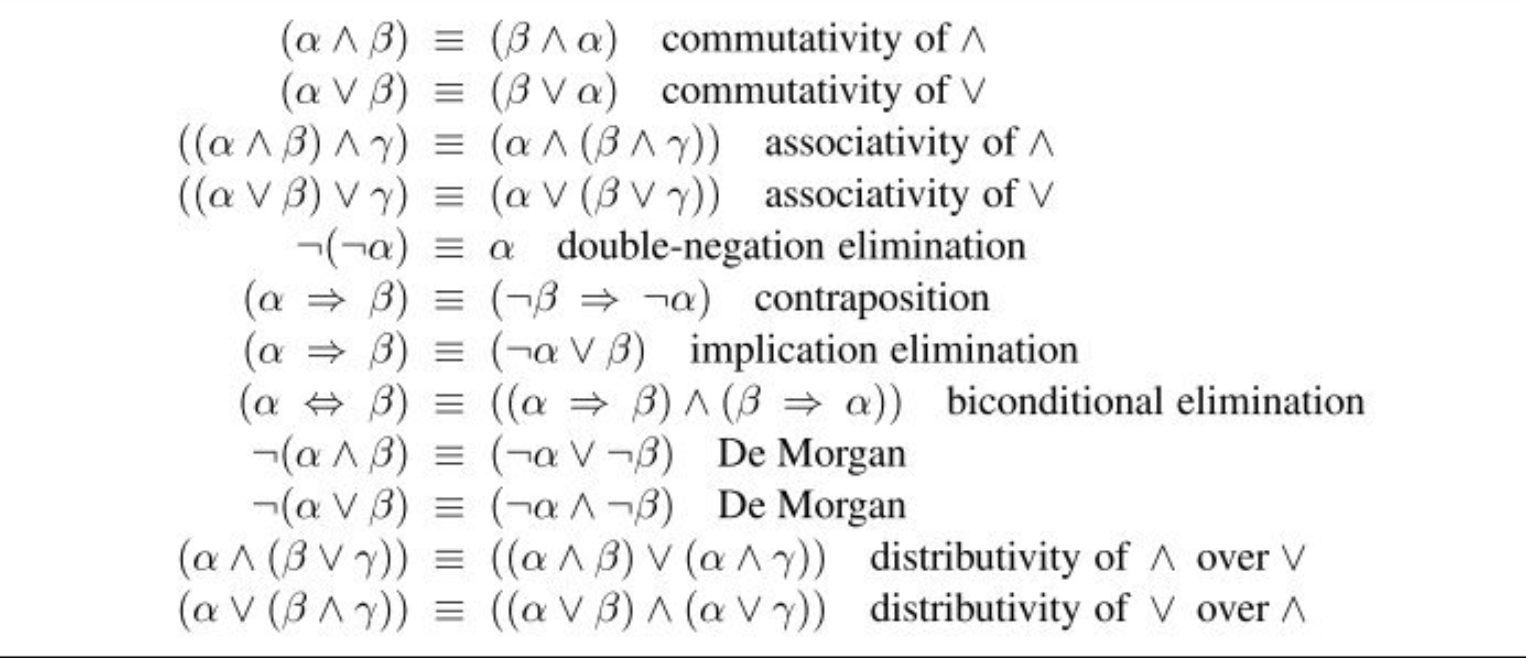
\includegraphics[width=8cm]{Standard Logical Equivalences.png}
\centering
\end{figure}

\subsubsection{Propositional Theorem Proving}

\textbf{Application of inference rules}

Legitimate (sound) generation of new sentences from old
Proof is a sequence of inference rule applications (Can use inference rules as operators in a standard search algorithm)
Typically require transformation of sentences into a normal form

\textbf{Model checking}

Truth table enumeration (always exponential in $n$)
Improved backtracking
Heuristic search in model space


\subsubsection{Propositional Inference}

There are two families of efficient algorithmns for propositional inference:
\begin{itemize}
    \item Complete backtracking search algorithms (DPLL algorithm)
    \item Incomplete local search algorithms (WalkSAT algorithm)
\end{itemize}

Both of these algorithmns manipulate formulae in \textbf{conjunctive normal form(CNF)}

In CNF a sentence is a conjunction of clauses whose satisfiability is to be determined. A clause is a disjuntion of literals and a literal is a proposition symbol.  \newline

To convert to CNF:
\begin{enumerate}
    \item Eliminate $\Leftrightarrow$: replace $\alpha \Leftrightarrow \beta$ with $(\alpha \Rightarrow \beta)\wedge(\beta \Rightarrow \alpha)$
    \item Eliminate $\Rightarrow$: replace $\alpha \Rightarrow \beta$ with $\neg \alpha \vee \beta$
    \item Move $\neg$ inwards: use de Morgan's rules and double negation $\neg \neg a = a$
    \item Create clauses: apply distributivity law $(\vee \: over \: \wedge)$ and flatten
\end{enumerate}

The original sentence is now in CNF, as a conjunction of clauses. 

\textbf{The DPLL algorithm} determines if an input propositional logic sentence (in CNF) is satisfiable

One component of DPLL is \textbf{early termination}:
\begin{itemize}
    \item A clause is true if one of its literals is true (E.g. if A is true then $A \vee \neg B$) is true
    \item A sentence is false if any of its clauses is false (e.g. If, A is false and B is true then ($A \vee B$) is false, so any sentence containing it is false)
\end{itemize}

Another aspect of DPLL is \textbf{Pure symbol heuristic}
\begin{itemize}
    \item Pure symbol: always appears with the same polarity in all clauses
    \item Make a literal containing a pure symbol true
\end{itemize}

The third component of DPLL is the \textbf{unit clause heuristic}
\begin{itemize}
    \item Unit clause: only one literal in the clause
    \item The only literal in a unit clause must be true
    \item Also includes clauses where all but one literal is false
\end{itemize}


\begin{algorithm}
\begin{algorithmic}

\Procedure{DPLL-SATISFIABLE}{$s$} 
\Comment{inputs: a sentence in propositional logic returns: true or false}
    \State $clauses \leftarrow$ the set of clauses in the CNF representation of $s$ 
    \State $symbols \leftarrow$ a list of the proposition symbols in $s$
    \State \textbf{return} DPLL($clauses,symbols,\{\}$) 
\EndProcedure \newline

\Procedure{DPLL}{$clauses,symbols,model$} \Comment{returns true or false}

    \If{every clause in $clauses$ is true in $model$} 
        \State \textbf{return} $true$
    \EndIf
    \If{some clauses in $clauses$ is false in $model$}
        \State \textbf{return} $false$
    \EndIf

    \State P,$value$ $\leftarrow$ FIND-PURE-SYMBOL($symbols,clauses,model$)
    \If{P is non-null}
        \State \textbf{return} DPLL($clauses,symbols -P, model \cup \{P=value\}$)
    \EndIf
    \State $P,value \leftarrow$ FIND-UNIT-CLAUSE($clauses,model$)
    \If{P is non-null}
        \State \textbf{return} DPLL($clauses,symbols-P,model \cup \{P = value\}$)
    \EndIf
    \State P$\leftarrow$ FIRST($symbols$); rest $\leftarrow$ REST($symbols$)

    \State \textbf{return} DPLL($clauses,rest,model \cup \{P=true\}$) or DPLL($clauses,rest,model \cup \{P=false\}$)

\EndProcedure

\end{algorithmic}
\end{algorithm}

\textbf{The WalkSat Algorithm} is an incomplete, local search algorithm. The evaluation function of WalkSat is the \textbf{min-conflict heuristic} of minimising the number of unsatisfied clauses.

The algorithm checks for satisfiability by randomly flipping the values of the variables. 

There is a balance between greediness and randomness \newline 

The below puesdocode for the algorithm takes the following inputs:
clauses, a set of clauses in propositional logic
p, the probability of choosing to do a "random walk" move, typically around 0.5
$maxFlips$, number of flips allowed before giving up \newline

And returns, a satisfying model or failure

\begin{algorithm}
\begin{algorithmic}

\Procedure{WALK-SAT}{$clauses,p,maxFlips$}
    \State $model \leftarrow$ a random assignment of $true/false$ to the symbols in $clauses$
    \For{$i = 1 \: to \: maxFlips$}

    \If{$model$ satisfies $clauses$}
        \State \textbf{return} $model$
    \EndIf

    \State $clause \leftarrow$ a randomly selected clause from $clauses$ that is false in $model$ with probability $p$ flip the value in $model$ of a randomly selected symbol from $clause$ otherwise flip whichever symbol in $clause$ maximises the number of satisfied clauses
    
    \EndFor
    \State \textbf{return} failure
\EndProcedure \newline

\end{algorithmic}
\end{algorithm}

\section{Resolution}

\subsection{Forward Chaining}

A forward-chaining algorithm starts with the atomic sentences in the knowledge base and applies Modus Ponenes in the forward direction, adding new atomic sentences, until no further inferences can be made. 

Properties of forward chaining:
\begin{itemize}
    \item Sound and complete for first-order definite clauses (a definite clause has exactly one positive literal)
    \item may not terminate in general if $\alpha$ is not entailed 
    \item Entailment with definite clauses is semi-decidable 
    \item Datalog = first-order definite clauses + no functions (FC terminates for Datalog in finite number of iterations)
\end{itemize}


\end{document}